% ---------
%  Compile with "pdflatex hw1".
% --------
%!TEX TS-program = pdflatex
%!TEX encoding = UTF-8 Unicode

% Template borrowed from Jeff Erickson.

\documentclass[11pt]{article}
\usepackage[utf8]{inputenc}		% Allow some non-ASCII Unicode in source
\usepackage{jeffe, handout,graphicx}
\usepackage{forest}
\usepackage{mathtools}
\usepackage{tikz, ifthen, etoolbox}
\usepackage{float}
\usetikzlibrary{positioning}
\newcommand{\pd}{\partial}
\newcommand{\bs}{\boldsymbol}
\newcommand{\ifstringequal}[4]{%
  \ifnum\pdfstrcmp{#1}{#2}=0
  #3%
  \else
  #4%
  \fi
}


% =========================================================
%   Define common stuff for solution headers
% =========================================================
\Class{CS 6301.503}
\Semester{Spring 2019}
\Authors{1}
\AuthorOne{Scott C. Waggener}{scw180000}
%\Section{}

% =========================================================
\begin{document}
\HomeworkHeader{6 (Design)}{1}% homework number, problem number
% ---------------------------------------------------------
Read
\begin{solution}
	Complete
\end{solution}

% =========================================================
\HomeworkHeader{6 (Design)}{2}% homework number, problem number
% ---------------------------------------------------------
Read
\begin{solution}
	Complete
\end{solution}

% =========================================================
\HomeworkHeader{6 (Design)}{3}% homework number, problem number
% ---------------------------------------------------------
Read
\begin{solution}
	Complete
\end{solution}

% =========================================================
\HomeworkHeader{6 (Design)}{4}% homework number, problem number
% ---------------------------------------------------------
Read
\begin{solution}
	Complete
\end{solution}

% =========================================================
\HomeworkHeader{6 (Design)}{5}% homework number, problem number
% ---------------------------------------------------------
Compute the receptive field size at the input to the global average pooling layer for ResNet 50.

\begin{solution}
	pass
\end{solution}
	Stride then add
\begin{proof}
	\begin{align}
		\bigg(
			\Big(
				\underbrace{1+2*3}_{\text{conv5}}
				+
				\underbrace{2*6}_{\text{conv4}}
				+
				\underbrace{2*4}_{\text{conv4}}
				+
				\underbrace{2*3}_{\text{conv4}}
			\Big)
			\underbrace{*2+2}_{\text{max pool}}
		\bigg)
		\underbrace{*2+6}_{\text{conv1}}
		\\
		=142
	\end{align}
\end{proof}

% =========================================================
\HomeworkHeader{6 (Design)}{6}% homework number, problem number
% ---------------------------------------------------------
\begin{enumerate}[(a)]
	\item How does the accuracy of the half wide version copare to the original
		version?
	\begin{solution}
		The accuracy at the final epoch for the full and half versions are
		\begin{align}
			\text{Full} &= 91.03\%
			&
			\text{Half} &= 89.31\%
		\end{align}
	\end{solution}
	\begin{proof}
	\end{proof}

	\item How long does an epoch of training take for both versions?
	\begin{solution}
		The times for epoch $3$ for both models (trained on GTX970) are
		\begin{align}
			\text{Full} &= 59s
			&
			\text{Half} &= 36s
		\end{align}
	\end{solution}
	\begin{proof}
	\end{proof}

	\item Approximate how feature map memory, filter memory, and compute change
		between the full and half width versions.
	\begin{solution}

		\begin{align}
			&\text{Feature map memory} = \frac{1}{2}
			\\
			&\text{Filter memory} = \frac{1}{2}
			\\
			&\text{Compute} = \frac{1}{4}
		\end{align}
	\end{solution}
	\begin{proof}
		As an approximation we can consider how CNN style 2D convolution layers
		will be impacted by the width reduction, as Resnet is primarily
		composed of such layers. For filter and feature map memory we will see
		a reduction approximately equal to the reduction in width. The
		dimensions of the filters and feature maps remain unchanged, but we are
		only considering half of the original feature maps and filters.
		\newline

		Recall that compute for CNN style 2D convolution depends on $N_o * N_i$
		which are both reduced by half, leading to a total reduction of $1/4$.
	\end{proof}

\end{enumerate}
% =========================================================
\HomeworkHeader{6 (Design)}{7}% homework number, problem number
% ---------------------------------------------------------
\begin{solution}
	The network design will be based on Inception v4. To inform our choice
	of network architecture we can use the given hint for an expected input
	global average pooling and think backwards from here. Obviously for
	CIFAR-10 we will have $10$ classes, so we need to choose $N_i$ to global
	average pooling somewhere above $10$, call it $50$.

\begin{figure}[H]
	\noindent\resizebox{\textwidth}{!}{
	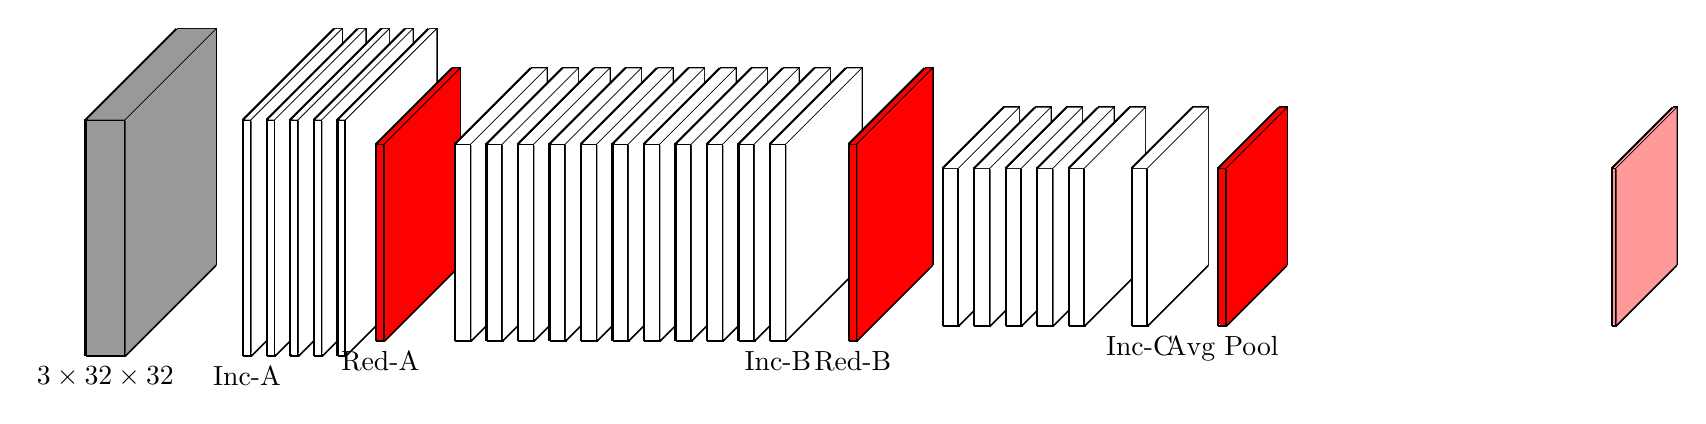
\begin{tikzpicture}

		% Define the macro.
		% 1st argument: Height and width of the layer rectangle slice.
		% 2nd argument: Depth of the layer slice
		% 3rd argument: X Offset --> use it to offset layers from previously drawn layers.
		% 4th argument: Options for filldraw.
		% 5th argument: Text to be placed below this layer.
		% 6th argument: Y Offset --> Use it when an output needs to be fed to
		%	multiple layers that are on the same X offset.

		\newcommand{\networkLayer}[6]{
			\def\a{#1} % Used to distinguish input resolution for current layer.
			\def\b{0.02}
			\def\c{#2} % Width of the cube to distinguish number of input channels for current layer.
			\def\t{#3} % X offset for current layer.
			\def\d{#4} % Y offset for current layer.

			% Draw the layer body.
			\draw[line width=0.3mm](\c+\t,0,\d)
				--(\c+\t,\a,\d)
				--(\t,\a,\d);
			\draw[line width=0.3mm](\t,0,\a+\d)
				--(\c+\t,0,\a+\d) node[midway,below] {#6}
				--(\c+\t,\a,\a+\d)
				--(\t,\a,\a+\d)
				--(\t,0,\a+\d);
			\draw[line width=0.3mm](\c+\t,0,\d) -- (\c+\t,0,\a+\d);
			\draw[line width=0.3mm](\c+\t,\a,\d) -- (\c+\t,\a,\a+\d);
			\draw[line width=0.3mm](\t,\a,\d) -- (\t,\a,\a+\d);

			% Recolor visible surfaces
			\filldraw[#5] (\t+\b,\b,\a+\d)
				--(\c+\t-\b,\b,\a+\d)
				--(\c+\t-\b,\a-\b,\a+\d)
				--(\t+\b,\a-\b,\a+\d)
				--(\t+\b,\b,\a+\d); % front plane
			\filldraw[#5] (\t+\b,\a,\a-\b+\d)
				--(\c+\t-\b,\a,\a-\b+\d)
				--(\c+\t-\b,\a,\b+\d)
				--(\t+\b,\a,\b+\d);

			% Colored slice.
			\ifthenelse {\equal{#5} {}}
			{} % Do not draw colored slice if #4 is blank.
			{\filldraw[#5] (\c+\t,\b,\a-\b+\d) --
				(\c+\t,\b,\b+\d) --
				(\c+\t,\a-\b,\b+\d) --
				(\c+\t,\a-\b,\a-\b+\d);
			} % Else, draw a colored slice.
		}

		\newcommand{\repeatLayer}[8]{
			% Repeat count
			% Spacing
		}

		% INPUT
		%\node[] (input image) at (-3.75,0.5) {\includegraphics[height=30mm]{lenna.png}};
		\networkLayer{3.0}{0.5}{-2}{0.0}{color=gray!80}{
			$3 \times 32 \times 32$
		}


		% ENCODER
		\networkLayer{3.0}{0.1}{0.0}{0.0}{color=white}{Inc-A}    % S1
		\foreach \i in {1,...,4}{
			\networkLayer{3.0}{0.1}{\i*0.3}
			{0.0}{color=white}{};
		}

		\networkLayer{2.5}{0.1}{1.5}{0.0}{color=red}{Red-A}    % S1

		\foreach \i in {0,...,9}{
			\networkLayer{2.5}{0.2}{2.5+0.4*\i}{0.0}
			{color=white}{}    % S1
		}
		\networkLayer{2.5}{0.2}{6.5}{0.0}{color=white}{Inc-B}    % S1

		\networkLayer{2.5}{0.1}{7.5}{0.0}{color=red}{Red-B}    % S1

		\foreach \i in {0,...,4}{
			\networkLayer{2}{0.2}{8.5+0.4*\i}{0.0}
			{color=white}{}    % S1
		}
		\networkLayer{2}{0.2}{10.9}{0.0}{color=white}{Inc-C}    % S1

		\networkLayer{2}{0.1}{12}{0.0}{color=red}{Avg Pool}    % S1

		% OUTPUT
		\networkLayer{2}{0.05}{17}{0.0}{color=red!40}{}          % Pixelwise segmentation with classes.
		%\node[] (output image) at (18,0.5) {\includegraphics[height=30mm]{vermeer.jpg}};


	\end{tikzpicture}
	}
	\caption{Example CNN.}
	\label{fig:cnn}
\end{figure}
\end{solution}
\begin{proof}
\end{proof}
% =========================================================
\HomeworkHeader{6 (Design)}{8}% homework number, problem number
% ---------------------------------------------------------
\begin{solution}
\end{solution}
\begin{proof}
\end{proof}
% =========================================================
\HomeworkHeader{6 (Design)}{9}% homework number, problem number
% ---------------------------------------------------------
\begin{solution}
\end{solution}
\begin{proof}
\end{proof}
\end{document}
